\documentclass{beamer}
\usepackage{amsmath}
\usepackage[english]{babel} %set language; note: after changing this, you need to delete all auxiliary files to recompile
\usepackage[utf8]{inputenc} %define file encoding; latin1 is the other often used option
\usepackage{csquotes} % provides context sensitive quotation facilities
\usepackage{graphicx} %allows for inserting figures
\usepackage{booktabs} % for table formatting without vertical lines
\usepackage{textcomp} % allow for example using the Euro sign with \texteuro
\usepackage{stackengine}
\usepackage{wasysym}
\usepackage{tikzsymbols}
\usepackage{textcomp}
% ELIMINAR COMANDOS DE NAVEGACION%%%%%%%%%%%
\setbeamertemplate{navigation symbols}

%\newcommand{\bubblethis}[2]{
 %       \tikz[remember picture,baseline]{\node[anchor=base,inner sep=0,outer sep=0]%
 %       (#1) {\underline{#1}};\node[overlay,cloud callout,callout relative pointer={(0.2cm,-0.7cm)},%
 %       aspect=2.5,fill=yellow!90] at ($(#1.north)+(-0.5cm,1.6cm)$) {#2};}%
 %   }%
%\tikzset{face/.style={shape=circle,minimum size=4ex,shading=radial,outer sep=0pt,
 %       inner color=white!50!yellow,outer color= yellow!70!orange}}

%% Some commands to make the code easier
\newcommand{\emoticon}[1][]{%
  \node[face,#1] (emoticon) {};
  %% The eyes are fixed.
  \draw[fill=white] (-1ex,0ex) ..controls (-0.5ex,0.2ex)and(0.5ex,0.2ex)..
        (1ex,0.0ex) ..controls ( 1.5ex,1.5ex)and( 0.2ex,1.7ex)..
        (0ex,0.4ex) ..controls (-0.2ex,1.7ex)and(-1.5ex,1.5ex)..
        (-1ex,0ex)--cycle;}
\newcommand{\pupils}{
  %% standard pupils
  \fill[shift={(0.5ex,0.5ex)},rotate=80] 
       (0,0) ellipse (0.3ex and 0.15ex);
  \fill[shift={(-0.5ex,0.5ex)},rotate=100] 
       (0,0) ellipse (0.3ex and 0.15ex);}

\newcommand{\emoticonname}[1]{
  \node[below=1ex of emoticon,font=\footnotesize,
        minimum width=4cm]{#1};}
\usepackage{scalerel}
\usetikzlibrary{positioning}
\usepackage{xcolor,amssymb}
\newcommand\dangersignb[1][2ex]{%
  \scaleto{\stackengine{0.3pt}{\scalebox{1.1}[.9]{%
  \color{red}$\blacktriangle$}}{\tiny\bfseries !}{O}{c}{F}{F}{L}}{#1}%
}
\newcommand\dangersignw[1][2ex]{%
  \scaleto{\stackengine{0.3pt}{\scalebox{1.1}[.9]{%
  \color{red}$\blacktriangle$}}{\color{white}\tiny\bfseries !}{O}{c}{F}{F}{L}}{#1}%
}
\usepackage{fontawesome} % Social Icons
\usepackage{epstopdf} % allow embedding eps-figures
\usepackage{tikz} % allows drawing figures
\usepackage{amsmath,amssymb,amsthm} %advanced math facilities
\usepackage{lmodern} %uses font that support italic and bold at the same time
\usepackage{hyperref}
\usepackage{tikz}
\hypersetup{
    colorlinks=true,
    linkcolor=blue,
    filecolor=magenta,      
    urlcolor=blue,
}
\usepackage{tcolorbox}
%add citation management using BibLaTeX
\usepackage[citestyle=authoryear-comp, %define style for citations
    bibstyle=authoryear-comp, %define style for bibliography
    maxbibnames=10, %maximum number of authors displayed in bibliography
    minbibnames=1, %minimum number of authors displayed in bibliography
    maxcitenames=3, %maximum number of authors displayed in citations before using et al.
    minnames=1, %maximum number of authors displayed in citations before using et al.
    datezeros=false, % do not print dates with leading zeros
    date=long, %use long formats for dates
    isbn=false,% show no ISBNs in bibliography (applies only if not a mandatory field)
    url=false,% show no urls in bibliography (applies only if not a mandatory field)
    doi=false, % show no dois in bibliography (applies only if not a mandatory field)
    eprint=false, %show no eprint-field in bibliography (applies only if not a mandatory field)
    backend=biber %use biber as the backend; backend=bibtex is less powerful, but easier to install
    ]{biblatex}
\addbibresource{../mybibfile.bib} %define bib-file located one folder higher


\usefonttheme[onlymath]{serif} %set math font to serif ones

\definecolor{beamerblue}{rgb}{0.2,0.2,0.7} %define beamerblue color for later use

%%% defines highlight command to set text blue
\newcommand{\highlight}[1]{{\color{blue}{#1}}}


%%%%%%% commands defining backup slides so that frame numbering is correct

\newcommand{\backupbegin}{
   \newcounter{framenumberappendix}
   \setcounter{framenumberappendix}{\value{framenumber}}
}
\newcommand{\backupend}{
   \addtocounter{framenumberappendix}{-\value{framenumber}}
   \addtocounter{framenumber}{\value{framenumberappendix}}
}

%%%% end of defining backup slides

%Specify figure caption, see also http://tex.stackexchange.com/questions/155738/caption-package-not-working-with-beamer
\setbeamertemplate{caption}{\insertcaption} %redefines caption to remove label "Figure".
%\setbeamerfont{caption}{size=\scriptsize,shape=\itshape,series=\bfseries} %sets figure  caption bold and italic and makes it smaller


\usetheme{Boadilla}

%set options of hyperref package
\hypersetup{
    bookmarksnumbered=true, %put section numbers in bookmarks
    naturalnames=true, %use LATEX-computed names for links
    citebordercolor={1 1 1}, %color of border around cites, here: white, i.e. invisible
    linkbordercolor={1 1 1}, %color of border around links, here: white, i.e. invisible
    colorlinks=true, %color links
    anchorcolor=black, %set color of anchors
    linkcolor=beamerblue, %set link color to beamer blue
    citecolor=blue, %set cite color to beamer blue
    pdfpagemode=UseThumbs, %set default mode of PDF display
    breaklinks=true, %break long links
    pdfstartpage=1 %start at first page
    }


% --------------------
% Overall information
% --------------------
\title[Economía I]{Economía I \vspace{4mm}
\\ Magistral 13: Competencia imperfecta}
\date{}
\author[Ertola Navajas y Fariña]{Ertola Navajas y Fariña}
\vspace{0.4cm}
\institute[]{Universidad de San Andrés} 

\begin{document}

\begin{frame}
\titlepage
\centering

\includegraphics[scale=0.2]{Slides Principios de Economia/Figures/logoUDESA.jpg} 
\end{frame}


\begin{frame}
\frametitle{El problema de la firma}
\begin{itemize}
    \item Una vez que conocemos la demanda... ¿cómo se elige cuánto producir y el precio que cobrar?
    \vspace{2mm}
    \item El problema principal de la empresa es el de la maximización del beneficio
    \vspace{2mm}     \begin{itemize}
        \item ¿Qué es el beneficio? \vspace{2mm} \\ 
        Beneficio = Ingresos totales – Costos totales
        \vspace{2mm}
        \item ¿Qué es el ingreso total? 
        \vspace{2mm} \\ 
        El valor de la producción al precio ofrecido (p·q)
        \vspace{2mm}
        \item ¿Qué es el costo total?
        \vspace{2mm} \\ 
        Los costos por unidad, por la cantidad de unidades producidas (c·q)
    \end{itemize} 
\end{itemize} 
\end{frame}

\begin{frame}
\frametitle{Monopolios}
\begin{itemize}
    \item Empresa que vende productos especializados tienen un alto poder de mercado\vspace{2mm}
    \begin{itemize}
        \item Enfrentan poca competencia, tienen una demanda inelástica, y pueden fijar precio superior al costo marginal sin perder todos sus clientes.\vspace{1mm}
        \item Las barreras de entrada ayudan a generar rentas \\
        - Beneficios económicos por encima de los costos de producción \\
        - Por eso las barreras a la entrada ¡son el peor enemigo de los economistas (y de la sociedad)!\vspace{4mm}
    \end{itemize}
    \item En estos casos, en equilibrio encontramos una pérdida de peso muerto
    \begin{itemize}
        \item Tenemos entonces una falla de mercado \\
        - Es decir, los mercados asignan recursos, sin competencia, en una forma no óptima 
    \end{itemize}
    \end{itemize}
\end{frame}


\begin{frame}
\frametitle{Mirando el ingreso total}
\begin{itemize}
    \item El concepto clave para la decisión del monopolista es el de ingreso marginal\vspace{2mm}
    \begin{itemize}
        \item Que es la variación en los ingresos totales al vender una unidad adicional.\vspace{1mm}
        \item Es el efecto neto de la disminución de los precios y el aumento de la cantidad vendida.\vspace{4mm}
    \end{itemize}
    \item La curva de demanda, veremos, nos determina ingresos marginales decrecientes\vspace{2mm}
    \begin{itemize}
        \item ¿Cómo cambia el ingreso al aumentar la producción? \\\vspace{1mm}
        - Ahora se vende una unidad más... \\
        - ...¡pero todas las vendo a un precio menor!
    \end{itemize}
\end{itemize}
\end{frame}

\begin{frame}
\frametitle{¿Cómo cambia el ingreso total?}
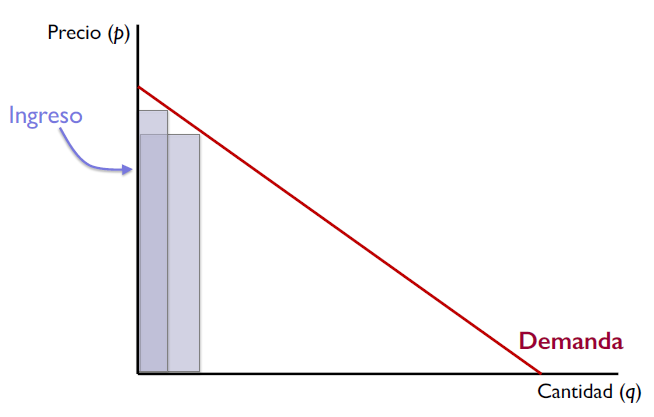
\includegraphics[scale=0.6]{Slides Principios de Economia/Figures/Tema_06.30_ingresototal.png}
\end{frame}

\begin{frame}
\frametitle{¿Cómo cambia el ingreso total?}
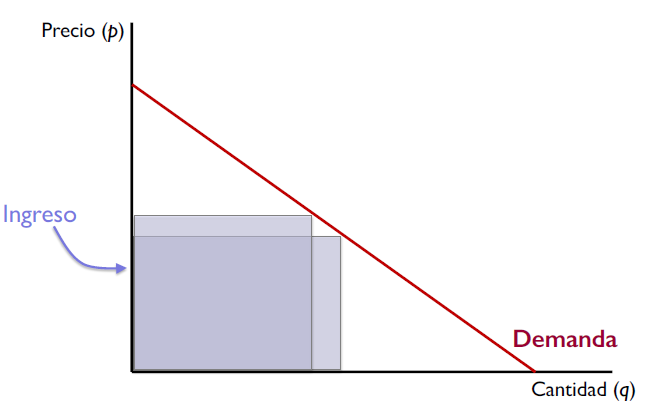
\includegraphics[scale=0.6]{Slides Principios de Economia/Figures/Tema_06.31_ingresototal2.png}
\end{frame}

\begin{frame}
\frametitle{¿Cómo cambia el ingreso total?}
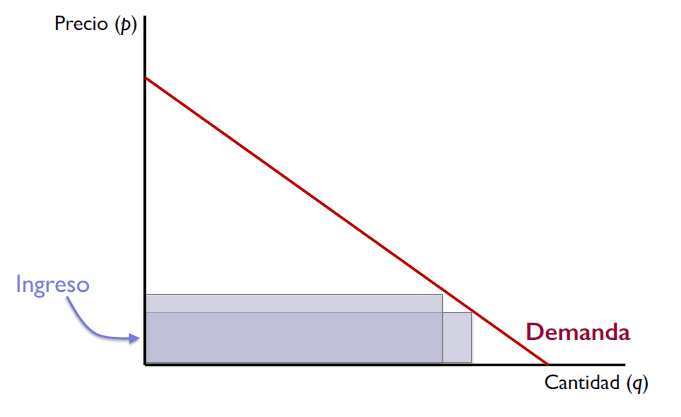
\includegraphics[scale=0.6]{Slides Principios de Economia/Figures/Tema_06.32_ingresototal3.png}
\end{frame}

\begin{frame}
\frametitle{El ingreso marginal}
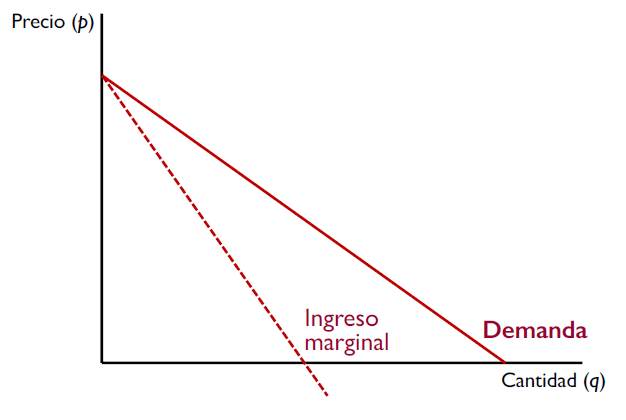
\includegraphics[scale=0.6]{Slides Principios de Economia/Figures/Tema_06.33_ingresomarginal.png}
\end{frame}

\begin{frame}
\frametitle{Costo e ingreso marginal}
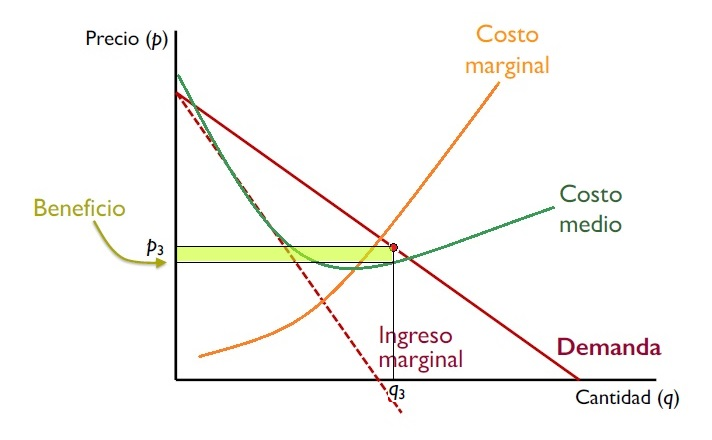
\includegraphics[scale=0.6]{Slides Principios de Economia/Figures/Tema_06.36_beneficios3.jpg}
\end{frame}

\begin{frame}
\frametitle{¿Cómo cambian los beneficios?}
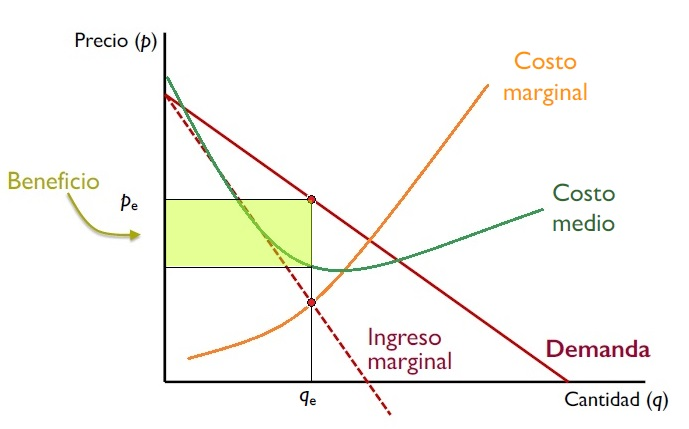
\includegraphics[scale=0.6]{Slides Principios de Economia/Figures/Tema_06.35_beneficios2.jpg}
\end{frame}

\begin{frame}
\frametitle{¿Cómo cambian los beneficios?}
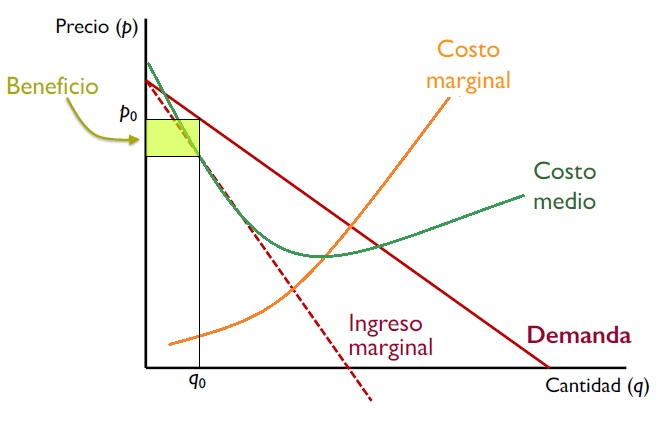
\includegraphics[scale=0.6]{Slides Principios de Economia/Figures/Tema_06.34_beneficios.jpg}
\end{frame}


\begin{frame}
\frametitle{La lógica marginal}
\begin{itemize}
    \item El punto que maximiza el beneficio es donde la curva de IMg cruza la curva de CMg\vspace{4mm}
    \item Recordemos que 
    b = p·q – C(q) = IT(q) - C(q)\vspace{2mm}
        \begin{itemize}
        \item Para cualquier valor de q, el cambio del beneficio si q fuera aumentado en una unidad sería la diferencia entre el cambio en ingresos, y el cambio en costos: \vspace{2mm} \\ \hspace{10mm}
    Beneficio marginal = IMg - CMg
        \vspace{2mm} \\
        \item Entonces: \\
            - Si $IMg > CMg$ aumentando q se podrían incrementar los beneficios \\
            - Si $IMg < CMg$ el beneficio marginal es negativo, con lo que sería mejor disminuir q para aumentar los beneficios
    \end{itemize}
    \end{itemize}
\end{frame}

\begin{frame}
\frametitle{Maximización de beneficios}
\begin{figure}[h!]
\centering
\scalebox{0.5}{
\tikzset{every picture/.style={line width=0.75pt}} %set default line width to 0.75pt        

\begin{tikzpicture}[x=0.75pt,y=0.75pt,yscale=-1,xscale=1]
%uncomment if require: \path (0,1344); %set diagram left start at 0, and has height of 1344

%Straight Lines [id:da18243805432710514] 
\draw    (202,871.69) -- (406,1108.5) ;
%Shape: Parabola [id:dp7498100266891665] 
\draw  [color={rgb, 255:red, 0; green, 0; blue, 0 }  ,draw opacity=1 ][line width=0.75]  (201,819.5) .. controls (269.33,562.42) and (337.67,562.42) .. (406,819.5) ;
%Straight Lines [id:da26559851992662464] 
\draw    (201,821.69) -- (472,821.69) ;
\draw [shift={(474,821.69)}, rotate = 180] [color={rgb, 255:red, 0; green, 0; blue, 0 }  ][line width=0.75]    (10.93,-3.29) .. controls (6.95,-1.4) and (3.31,-0.3) .. (0,0) .. controls (3.31,0.3) and (6.95,1.4) .. (10.93,3.29)   ;
%Straight Lines [id:da5363525623734258] 
\draw    (201,1107.69) -- (472,1107.69) ;
\draw [shift={(474,1107.69)}, rotate = 180] [color={rgb, 255:red, 0; green, 0; blue, 0 }  ][line width=0.75]    (10.93,-3.29) .. controls (6.95,-1.4) and (3.31,-0.3) .. (0,0) .. controls (3.31,0.3) and (6.95,1.4) .. (10.93,3.29)   ;
%Straight Lines [id:da3817553551786188] 
\draw    (201,821.69) -- (201,591.69) ;
\draw [shift={(201,589.69)}, rotate = 450] [color={rgb, 255:red, 0; green, 0; blue, 0 }  ][line width=0.75]    (10.93,-3.29) .. controls (6.95,-1.4) and (3.31,-0.3) .. (0,0) .. controls (3.31,0.3) and (6.95,1.4) .. (10.93,3.29)   ;
%Straight Lines [id:da7748677219246147] 
\draw    (201,1107.69) -- (200.01,854.69) ;
\draw [shift={(200,852.69)}, rotate = 449.78] [color={rgb, 255:red, 0; green, 0; blue, 0 }  ][line width=0.75]    (10.93,-3.29) .. controls (6.95,-1.4) and (3.31,-0.3) .. (0,0) .. controls (3.31,0.3) and (6.95,1.4) .. (10.93,3.29)   ;
%Shape: Circle [id:dp8783199097392036] 
\draw  [fill={rgb, 255:red, 0; green, 0; blue, 0 }  ,fill opacity=1 ] (300.72,627.58) .. controls (300.1,626.08) and (300.85,624.47) .. (302.39,623.98) .. controls (303.92,623.49) and (305.67,624.3) .. (306.28,625.8) .. controls (306.9,627.3) and (306.15,628.91) .. (304.61,629.4) .. controls (303.08,629.89) and (301.33,629.07) .. (300.72,627.58) -- cycle ;
%Straight Lines [id:da4368467901848765] 
\draw    (202,871.69) -- (362,1231.69) ;
%Straight Lines [id:da5238163933422064] 
\draw    (303.5,626.69) -- (305,1107.69) ;
%Shape: Circle [id:dp1228744006153617] 
\draw  [fill={rgb, 255:red, 0; green, 0; blue, 0 }  ,fill opacity=1 ] (301.22,990.98) .. controls (300.6,989.49) and (301.35,987.87) .. (302.89,987.38) .. controls (304.42,986.89) and (306.17,987.71) .. (306.78,989.2) .. controls (307.4,990.7) and (306.65,992.31) .. (305.11,992.8) .. controls (303.58,993.3) and (301.83,992.48) .. (301.22,990.98) -- cycle ;
%Shape: Circle [id:dp15078348251983176] 
\draw  [fill={rgb, 255:red, 0; green, 0; blue, 0 }  ,fill opacity=1 ] (302.22,1108.58) .. controls (301.6,1107.08) and (302.35,1105.47) .. (303.89,1104.98) .. controls (305.42,1104.49) and (307.17,1105.3) .. (307.78,1106.8) .. controls (308.4,1108.3) and (307.65,1109.91) .. (306.11,1110.4) .. controls (304.58,1110.89) and (302.83,1110.07) .. (302.22,1108.58) -- cycle ;
%Straight Lines [id:da3583437704153747] 
\draw    (201,989.69) -- (304,990.09) ;
%Straight Lines [id:da11618331349069289] 
\draw    (202,626.69) -- (303.5,626.69) ;

% Text Node
\draw (474,1119.69) node [anchor=north west][inner sep=0.75pt]   [align=left] {Q};
% Text Node
\draw (474,821.69) node [anchor=north west][inner sep=0.75pt]   [align=left] {Q};
% Text Node
\draw (138,556.69) node [anchor=north west][inner sep=0.75pt]   [align=left] {\begin{minipage}[lt]{39.58pt}\setlength\topsep{0pt}
\begin{center}
Ingreso \\total
\end{center}

\end{minipage}};
% Text Node
\draw (150,832.69) node [anchor=north west][inner sep=0.75pt]   [align=left] {Precio};
% Text Node
\draw (177,978.69) node [anchor=north west][inner sep=0.75pt]   [align=left] {P{\scriptsize E}};
% Text Node
\draw (294,822.69) node [anchor=north west][inner sep=0.75pt]   [align=left] {Q{\scriptsize E}};
% Text Node
\draw (407,1083.69) node [anchor=north west][inner sep=0.75pt]   [align=left] {D};
% Text Node
\draw (409,785.69) node [anchor=north west][inner sep=0.75pt]   [align=left] {IT};
% Text Node
\draw (343,1160.69) node [anchor=north west][inner sep=0.75pt]   [align=left] {IMg};
% Text Node
\draw (298,602) node [anchor=north west][inner sep=0.75pt]   [align=left] {{\footnotesize E}};
% Text Node
\draw (291,1108.69) node [anchor=north west][inner sep=0.75pt]   [align=left] {Q{\scriptsize E}};
% Text Node
\draw (306,967) node [anchor=north west][inner sep=0.75pt]   [align=left] {{\footnotesize E}};
% Text Node
\draw (137,606.69) node [anchor=north west][inner sep=0.75pt]   [align=left] {Ingreso \ \\máximo};


\end{tikzpicture}
}
\end{figure}
\end{frame}




\begin{frame}
\frametitle{Excedentes y peso muerto}
\begin{itemize}
    \item Las ganancias totales del intercambio están determinadas por los excedentes de consumidores y productores\vspace{2mm}
    \begin{itemize}
        \item El excedente del consumidor \\ - Diferencia entre disposición a pagar y precio de compra\vspace{1mm}
        \item Excedente del productor \\ - Diferencia entre precio y costo de una unidad adicional\vspace{4mm}
    \end{itemize}
    \item Si no terminamos en una asignación Pareto eficiente tenemos una ‘pérdida de peso muerto’\vspace{2mm}
    \begin{itemize}
        \item Pérdida de excedente total con respecto a una asignación eficiente de Pareto \\
        - Es decir, hay ganancias no explotadas del comercio
    \end{itemize}
    \end{itemize}
\end{frame}

%\begin{frame}
%\frametitle{Precios y excedentes}
%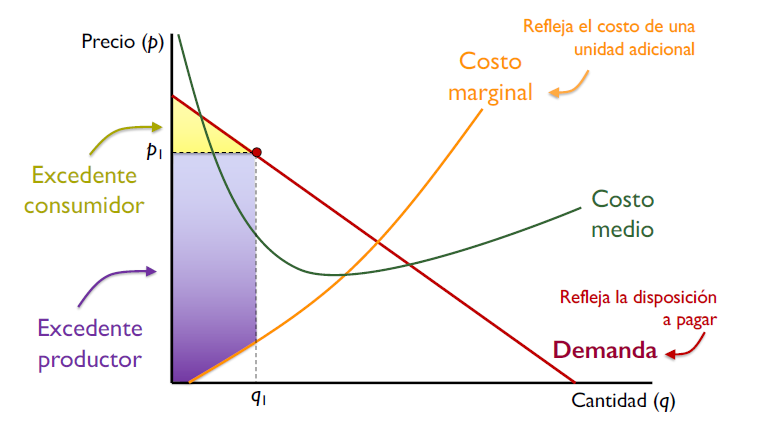
\includegraphics[scale=0.6]{Slides Principios de Economia/Figures/Tema_06.38_excedente1.png}
%\end{frame}

%\begin{frame}
%\frametitle{Mejora de Pareto}
%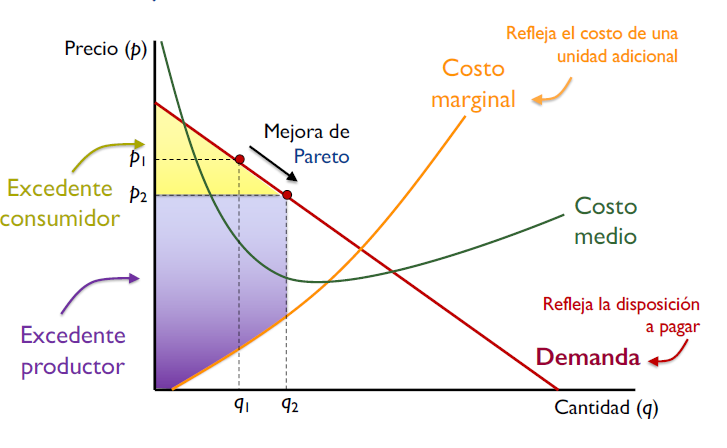
\includegraphics[scale=0.6]{Slides Principios de Economia/Figures/Tema_06.39_excedente2.png}
%\end{frame}

\begin{frame}
\frametitle{Eficiencia de Pareto}
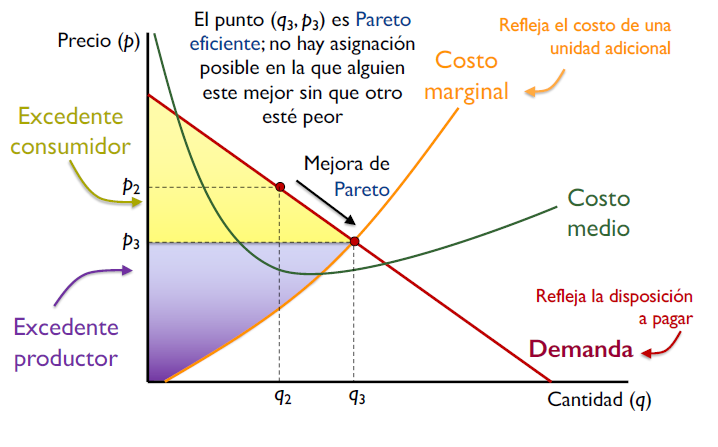
\includegraphics[scale=0.6]{Slides Principios de Economia/Figures/Tema_06.40_excedente3.png}
\end{frame}

\begin{frame}
\frametitle{Cuando maximiza la firma}
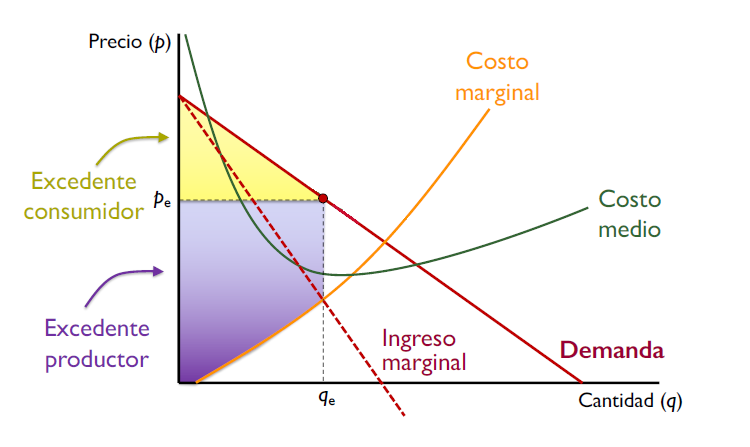
\includegraphics[scale=0.6]{Slides Principios de Economia/Figures/Tema_06.41_excedente4.png}
\end{frame}

\begin{frame}
\frametitle{Pérdida de eficiencia}
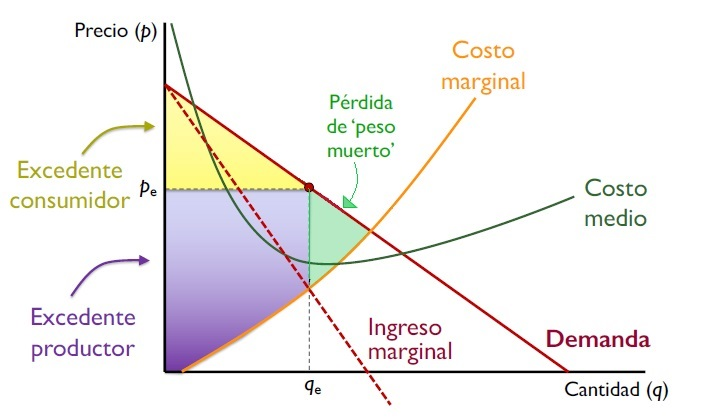
\includegraphics[scale=0.6]{Slides Principios de Economia/Figures/Tema_06.42_excedente5.jpg}
\end{frame}

\begin{frame}
\frametitle{Elasticidad y maximización}
\begin{itemize}
    \item Claramente, la firma va a elegir un nivel de producción en la parte elástica de la demanda\vspace{2mm}
    \begin{itemize}
        \item Cuando en la parte inelástica, $IMg < 0$, con lo cual se puede estar mejor reduciendo la producción\vspace{4mm}
    \end{itemize}
    \item La elasticidad precio de la demanda afecta el margen de beneficio $(p – CMg)$ de la empresa\vspace{2mm}
    \begin{itemize}
        \item Cuanto mas elástica es la curva, menos margen, y menor la perdida de peso muerto \\
        - Pequeños cambios en precios $\rightarrow$ gran diferencia en ventas
        \item El markup (margen de ganancia como \% del precio) es inversamente proporcional a la elasticidad precio de la demanda
    \end{itemize}
\end{itemize}
\end{frame}

\begin{frame}
\frametitle{Demanda más elástica}
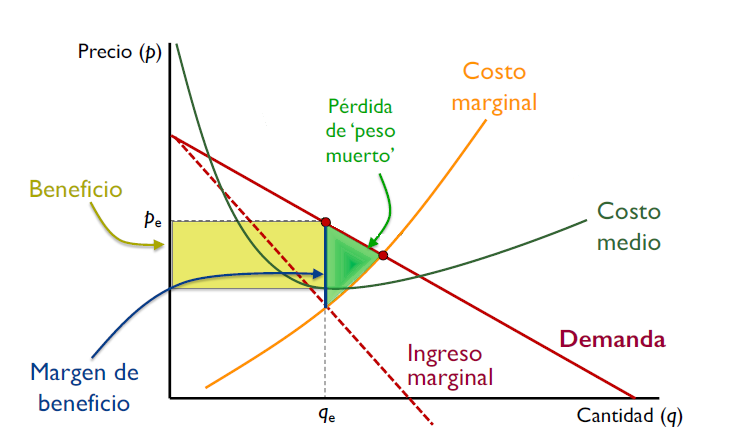
\includegraphics[scale=0.6]{Slides Principios de Economia/Figures/Tema_06.47_elasticidad3.png}
\end{frame}

\begin{frame}
\frametitle{Demanda más inelástica}
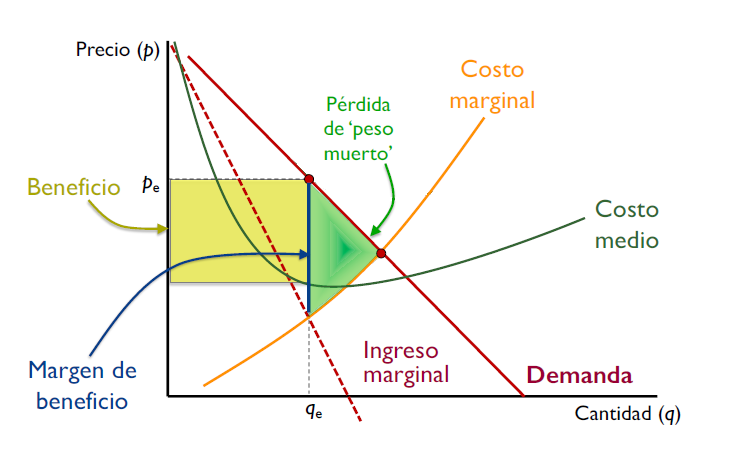
\includegraphics[scale=0.6]{Slides Principios de Economia/Figures/Tema_06.48_elasticidad4.png}
\end{frame}

\begin{frame}
\frametitle{Poder de mercado}
\begin{itemize}
    \item El margen de beneficio de una empresa depende de la elasticidad de la demanda\vspace{2mm}
    \begin{itemize}
        \item Esta, a su vez se ve afectada por la competencia: \\
        - Demanda relativamente inelástica si hay pocos sustitutos. \\
        - Las empresas con poder de mercado tienen suficiente poder de negociación para fijar los precios sin perder clientes a los competidores.\vspace{4mm}
    \end{itemize}
    \item La política de competencia (antitrust), que limita el poder de mercado, puede beneficiar a los consumidores\vspace{2mm}
    \begin{itemize}
        \item Por ejemplo, cuando empresas se pueden agrupar en un cartel (poniéndose de acuerdo para mantener precios altos)
    \end{itemize}
\end{itemize}
\end{frame}

\begin{frame}
\frametitle{Ganando poder de mercado}
\begin{itemize}
    \item ¿Cómo aumentar el poder de mercado?\vspace{2mm}
    \begin{itemize}
        \item La innovación tecnológica permite diferenciar los productos \\
        - Una empresa que inventan un producto completamente nuevo pueden prevenir la competencia por completo a través de patentes o las leyes de copyright\vspace{1mm}
        \item Con la publicidad las empresas pueden atraer a los consumidores, alejándolos de la competencia y creando lealtad a la marca \\      - Puede ser más eficaz que los descuentos en el aumento de la demanda de una marca\vspace{4mm}
        \end{itemize}
        \item Ambas tácticas pueden cambiar la curva de demanda que enfrenta la empresa
\end{itemize}
\end{frame}

\begin{frame}
\frametitle{Monopolios naturales}
\begin{itemize}
    \item Hay casos en los cuales el poder monopólico surge de características tecnológicas, de estructura de costos\vspace{2mm}
    \begin{itemize}
        \item Cuando el costo medio es decreciente \\
        - Economías de escala, altos costos fijos, o precios de factores que caen cuanto mas compra la empresa.\vspace{1mm}
        \item La empresa debe elegir un precio al menos igual al costo medio, que es más alto que el costo marginal \\
        - ¿Por qué?\vspace{4mm}
        \end{itemize}
    \item En estos casos tenemos un monopolio natural\vspace{2mm}
    \begin{itemize}
        \item En estos casos, en lugar de fomentar la competencia, el gobierno suele poner controles de precios o hacer estas empresas de propiedad pública
    \end{itemize}
    \end{itemize}
\end{frame}

\begin{frame}
\frametitle{Casos ideales}
\small
\begin{center}
    \begin{tabular}{c|c}
    \hline
    \hline
    Tomadores de precios & Fijadores de precio \\
    Competencia Perfecta & Monopolio
    \\
    \hline
    \hline
    Puede ser   & Pareto ineficiente \\ 
    Pareto eficiente & (pérdidas peso muerto)
    \\
    \hline
    No hay rentas & Rentas económicas \\
    económicas en & tanto a largo \\
    el largo plazo & como a corto plazo
    \\
    \hline
    Poca gasto en su & Firmas publicitan \\ publicidad & producto único 
    \\
    \hline
    Pocos incentivos para & Firmas invierten en IyD \\ 
    la innovación porque & (tratan de evitar ser \\
    porque otras van a copiar & copiadas)
\end{tabular}
\end{center}
\end{frame}

\begin{frame}
\frametitle{Competencia imperfecta}
\begin{itemize}
    \item La empresa típica se ubica en algún punto entre los casos extremos de la competencia perfecta y el monopolio \vspace{4mm}
    \item Mercados de competencia imperfecta \vspace{2mm}
    \begin{itemize}
        \item Oligopolio: sólo hay pocos vendedores, cada uno de los cuales ofrece un producto idéntico o similar a los productos ofrecidos por otros vendedores
        \item Competencia monopolística: existen numerosas empresas que venden productos similares, pero no idénticos porque logran diferenciarse
    \end{itemize}
    \end{itemize}
\end{frame}

\begin{frame}
\frametitle{Determinantes de la concentración}
\begin{itemize}
    \item Costos
        \begin{itemize}
        \item La existencia de economías de escala hace que solo sobrevivan en el mercado pocas empresas produciendo una gran parte de lo que demanda el mercado 
        \end{itemize}
    \vspace{2mm}
    \item Barreras a la entrada 
        \begin{itemize}
        \item Cuando hay barreras a la entrada se bloquea el acceso para que otros empresas ingresen al mercado
        \end{itemize}
    \vspace{2mm}
    \item Interdependencia estratégica
        \begin{itemize}
        \item Cuando las decisiones de una empresa dependen de las decisiones que toman otras empresas 
        \end{itemize}
    \end{itemize}
\end{frame}

\begin{frame}
\frametitle{Oligopolio}
\begin{itemize}
    \item Competencia entre unas pocas empresas. \vspace{4mm}
    \item Obliga a las empresas a tener en cuenta las reacciones de las competidoras a las desviaciones de los precios de los niveles de producción.\vspace{4mm}
    \item Se introducen consideraciones estratégicas en sus mercados.
\end{itemize}
\end{frame}

\begin{frame}
\frametitle{¿Cómo compiten pocas empresas?}
\begin{itemize}
    \item Modelo de Cournot: las empresas eligen cantidades de manera simultánea. \vspace{2mm}
    \item Modelo de Bertrand: las empresas deciden el precio que establecen y lo hacen de manera simultánea.  \vspace{2mm}
    \item Colusión: las empresas eligen precio o cantidad de manera simultánea pero coordinada, es decir, poniéndose de acuerdo. Ejemplo: OPEP y Beers.
    \item Modelo de líder y seguidores: en este caso la competencia es secuencial, es decir, una empresa líder decide primero y luego los seguidores observan la acción y eligen su respuesta. Por ejemplo, precios establecidos por Mc Donald´s y Burger King. Las empresas pueden elegir precios o cantidades.
\end{itemize}
\end{frame}

\begin{frame}
\frametitle{Veamos un ejemplo}
\centering
\begin{table}
\begin{tabular}{|c|c|c|c|}
\hline
\multicolumn{2}{|c|}{}                                     & \multicolumn{2}{c|}{\textbf{Empresa B}}              \\ \cline{3-4} 
\multicolumn{2}{|c|}{\multirow{}{}{\textbf{}}}          & \textbf{Producción Alta}           & \textbf{Producción Baja} \\ \hline
                                   & \textbf{Producción Alta} & {\color[HTML]{000000} 1.600 ; 1.600} & 2.000 ; 1.500            \\ \cline{2-4} 
\multirow{}{}{\textbf{Empresa A}} & \textbf{Producción Baja}    & 1.500 ; 2.000                         & 1.800 ; 1.800           \\ \hline
\end{tabular}
\end{table}
\end{frame}


\begin{frame}
\frametitle{Cartel}
\begin{itemize}
    \item Es una organización de empresas independientes, que producen bienes similares.\vspace{4mm}
    \item Trabajan conjuntamente para elevar los precios y restringir la producción.\vspace{4mm}
    \item Se comportan como un monopolista.\vspace{4mm}
    \item Colusión explicita versus colusión tácita.\vspace{4mm}
    \end{itemize}
\end{frame}


%\begin{frame}
%\frametitle{La maximización de beneficios del Cartel}
%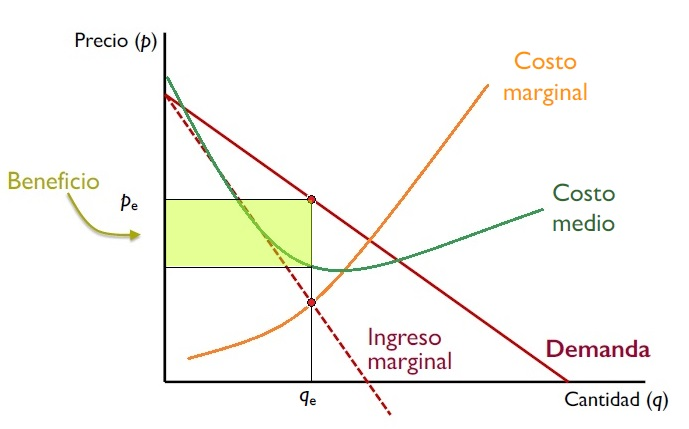
\includegraphics[scale=0.6]{Slides Principios de Economia/Figures/Tema_06.35_beneficios2.jpg}
%\end{frame}

\begin{frame}
\frametitle{Obstáculos para el cartel}
\begin{itemize}
    \item Son ilegales.\vspace{4mm}
    \item Hay incentivos para romper los acuerdos\vspace{2mm}
    \begin{itemize}
        \item Cobrando un precio apenas más bajo, una empresa aumentando su participación de mercado y saca enormes beneficios.\vspace{1mm}
        \item Esto sucede porque la demanda individual es elástica.
    \end{itemize}
   % \item Hoy en día hay una fuerte competencia procedente de empresas extranjeras además de las nacionales
\end{itemize}
\end{frame}

\begin{frame}
\frametitle{El caso de las cementeras}
\centering

\includegraphics[width=0.95\textwidth]{Slides Principios de Economia/Figures/Cartel.png}

\end{frame}

\begin{frame}
\frametitle{Competencia monopolística}
\begin{center}
  \href{https://www.youtube.com/watch?v=po0jY4WvCIc}{    
\includegraphics[width=0.75\textwidth]{Slides Principios de Economia/Figures/Diferenciacion (1).png}}
\end{center}
\end{frame}

\begin{frame}
\frametitle{Competencia monopolística}
\begin{itemize}
    \item Hay muchos compradores y vendedores\vspace{2mm}
    \item Es fácil entrar y salir\vspace{2mm}
    \item Las empresas toman los precios de las demás como dados\vspace{2mm}
    \item Los productos están diferenciados\vspace{2mm}
    \begin{itemize}
        \item Cada vendedor tiene libertad para subir o bajar los precios debido a la diferenciación de productos.\vspace{1mm}
        \item Entonces, la curva de demanda de cada vendedor tenga pendiente negativa.
    \end{itemize}
    \end{itemize}
\end{frame}

\begin{frame}
\frametitle{La maximización de beneficios en Competencia Monopolística en corto plazo}
%\centering
%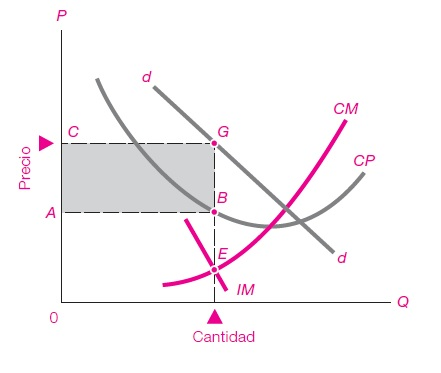
\includegraphics[scale=0.75]{Slides Principios de Economia/Figures/Tema_08.01_compmonop.jpg}

\begin{figure}[h!]
\renewcommand{\figurename}{Figure}

%\tikzset{every picture/.style={line width=0.75pt}} %set default line width to 0.75pt        
\begin{center}
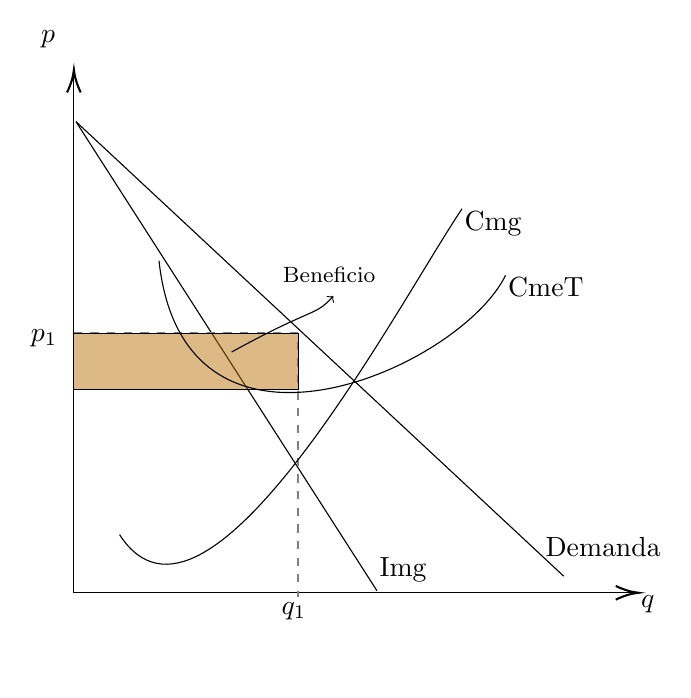
\begin{tikzpicture}[x=0.75pt,y=0.75pt,yscale=-1,xscale=1]
% \path (0,1278); %set diagram left start at 0, and has height of 1278

%Straight Lines Eje
\draw    (94,318) -- (364,318) ;
\draw [shift={(366,318)}, rotate = 180] [color={rgb, 255:red, 0; green, 0; blue, 0 }  ][line width=0.75]    (10.93,-3.29) .. controls (6.95,-1.4) and (3.31,-0.3) .. (0,0) .. controls (3.31,0.3) and (6.95,1.4) .. (10.93,3.29)   ;
%Straight Lines: Eje
\draw    (94,318) -- (94,68) ;
\draw [shift={(94,66)}, rotate = 450] [color={rgb, 255:red, 0; green, 0; blue, 0 }  ][line width=0.75]    (10.93,-3.29) .. controls (6.95,-1.4) and (3.31,-0.3) .. (0,0) .. controls (3.31,0.3) and (6.95,1.4) .. (10.93,3.29)   ;

% Membrete eje Y
\draw (77,46) node [anchor=north west][inner sep=0.75pt]   [align=left] {$p$};
% Membrete eje X
\draw (366,318) node [anchor=north west][inner sep=0.75pt]   [align=left] {$q$};


% AR 
\draw    (95,91) -- (330,310) ;
\draw (320,290) node [anchor=north west][inner sep=0.75pt]   [align=left] {Demanda};
% Img (MR)
\draw    (95,91) -- (240,317) ;
\draw (240,300) node [anchor=north west][inner sep=0.75pt]   [align=left] {Img};
% dash lines
\draw[thick, dashed, gray] (94,193)-- (202,193) -- (202,320);
\node [below] at (200,318) {$q_1$};
%Shape: Rectangle profit
\draw  [fill={rgb:red,4;green,2;yellow,1 }  ,fill opacity=0.48 ] (94,193) -- (202,193) -- (202,220) -- (94,220) ;
\draw (72,190) node [anchor=north west][inner sep=0.75pt]   [align=left] {$p_1$};
%Curve Lines Cme T 
\draw    (135,158) .. controls (147,269) and (280,210) .. (302,165) ;
\draw (302,165) node [anchor=north west][inner sep=0.75pt]   [align=left] {CmeT};
% curve line Cmg
\draw    (116,290) .. controls (158,355) and (250,179) .. (281,133) ;
\draw (281,133) node [anchor=north west][inner sep=0.75pt]   [align=left] {Cmg};

% short run equilibrium

\draw[thin, ->] (170,202).. controls (210,180) and         (210,185)..(219,175);
\node[right] at (190,165) {\footnotesize Beneficio};

\end{tikzpicture}
\end{center}
\end{figure}
\end{frame}

\begin{frame}
\frametitle{Competencia monopolística en el largo plazo}
\begin{itemize}
    \item Los beneficios positivos en el corto plazo atraen nuevas empresas.\vspace{2mm}
    \item La demanda que enfrenta la empresa se contrae.\vspace{2mm}
    \item Los precios son superiores a los costos marginales.\vspace{2mm}
    \item En el largo plazo, los beneficios de la empresa son iguales a cero, es decir, tiene beneficios normales.
\end{itemize}
\end{frame}

\begin{frame}
\frametitle{La maximización de beneficios en Competencia Monopolística en largo plazo}
%\centering
%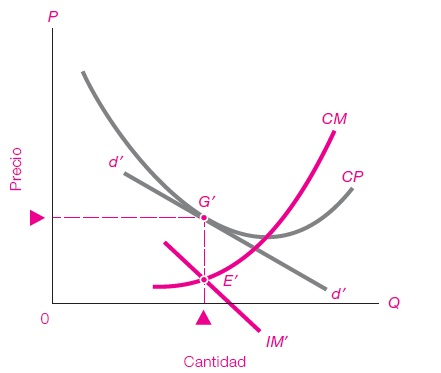
\includegraphics[scale=0.7]{Slides Principios de Economia/Figures/Tema_08.02_compmonop.jpg}

\begin{figure}[H]
\renewcommand{\figurename}{Figure}
%\begin{tikzpicture}[scale=0.45]
%\centering
%\tikzset{every picture/.style={line width=0.75pt}} %set default line width to 0.75pt        
\begin{center}
\begin{tikzpicture}[x=0.75pt,y=0.75pt,yscale=-1,xscale=1]
% \path (0,1278); %set diagram left start at 0, and has height of 1278

%Straight Lines [id:da6898288131267385] 
\draw    (94,318) -- (364,318) ;
\draw [shift={(366,318)}, rotate = 180] [color={rgb, 255:red, 0; green, 0; blue, 0 }  ][line width=0.75]    (10.93,-3.29) .. controls (6.95,-1.4) and (3.31,-0.3) .. (0,0) .. controls (3.31,0.3) and (6.95,1.4) .. (10.93,3.29)   ;
%Straight Lines [id:da9536118190051617] 
\draw    (94,318) -- (94,68) ;
\draw [shift={(94,66)}, rotate = 450] [color={rgb, 255:red, 0; green, 0; blue, 0 }  ][line width=0.75]    (10.93,-3.29) .. controls (6.95,-1.4) and (3.31,-0.3) .. (0,0) .. controls (3.31,0.3) and (6.95,1.4) .. (10.93,3.29)   ;
% AR 
\draw    (95,91) -- (201,317) ;
\draw (200,300) node [anchor=north west][inner sep=0.75pt]   [align=left] {Demanda};
% Img (MR)
\draw    (95,91) -- (150,317) ;
\draw (155,300) node [anchor=north west][inner sep=0.75pt]   [align=left] {Img};
% dash lines
\draw[thick, dashed, gray] (94,191)-- (146,191) -- (146,320);
\node [below] at (146,318) {$q_1$};
\draw (72,191) node [anchor=north west][inner sep=0.75pt]   [align=left] {$p_1$};
%Shape: Rectangle profit
%\draw  [fill={rgb:red,4;green,2;yellow,1 }  ,fill opacity=0.48 ] (94,193) -- (202,193) -- (202,220) -- (94,220) ;


%Curve Lines Cme T 
% MAS ALEJADA LA CME T
%\draw    (180,128) .. controls (147,200) and (280,210) .. (302,165) ;
%\draw (302,165) node [anchor=north west][inner sep=0.75pt]   [align=left] {CmeT};
% MISMA QUE LA DE SHORT RUN
\draw    (135,158) .. controls (147,269) and (280,210) .. (302,165) ;
\draw (302,165) node [anchor=north west][inner sep=0.75pt]   [align=left] {CmeT};

% curve line Cmg
\draw    (116,290) .. controls (158,355) and (250,179) .. (281,133) ;
\draw (281,133) node [anchor=north west][inner sep=0.75pt]   [align=left] {Cmg};

% Text Node
\draw (77,46) node [anchor=north west][inner sep=0.75pt]   [align=left] {$p$};
% Text Node
\draw (366,318) node [anchor=north west][inner sep=0.75pt]   [align=left] {$q$};

% Long run equilibrium
\draw[thin, ->] (150,191).. controls (190,160) and         (210,125)..(210,125);
\node[right] at (200,100) {\footnotesize Equilibrio de};
\node[right] at (200,115) {\footnotesize largo plazo};

\end{tikzpicture}
\end{center}
\end{figure}

\end{frame}
\end{document}
